\subsection{Wanderjahre}

\hypertarget{RefHeadingToc100333728}{}Nach seinem Abschluss, dem
sogenannten „Absolutorium“, an der Lehrerbildungsanstalt in Straubing
1898, absolvierte August Högn an seiner ehemaligen Knabenschule in
Deggendorf ein Praktikum bei den Lehrern Buchner und Edelmann. Als
Aushilfslehrer waren seine Stationen Neukirchen bei Haggn im Landkreis
Straubing-Bogen, Schaufling bei Deggendorf und Geratskirchen in der
Nähe von Eggenfelden. Im Rang eines Hilfslehrers unterrichtete er in
Zeilarn bei Simbach am Inn und Wallersdorf. 1902 legte er an der
Regierung von Niederbayern die Anstellungsprüfung ab und wurde ab 1.
Januar 1903 Schulverweser in Wallersdorf. \footnote{Dokument Nr. 48,
Zeitungsartikel aus Viechtacher Bayerwald-Bote, 2.8.1958}
„Schulverweser“ ist eine 1896 eingeführte Bezeichnung für den
Schulgehilfen, also den zweiten Lehrer und Vertreter des
Schulleiters.\footnote{
http://www.markt-pfaffenhofen.de/geschichte/html\_geschichte/die\_schulverweser\_in\_pfaffenhofen.htm}
Dort lernte er seine Ehefrau Emma kennen.

\begin{flushleft}
\tablefirsthead{}
\tablehead{}
\tabletail{}
\tablelasttail{}
\begin{supertabular}{m{4.3650002cm}m{4.894cm}m{6.556cm}}

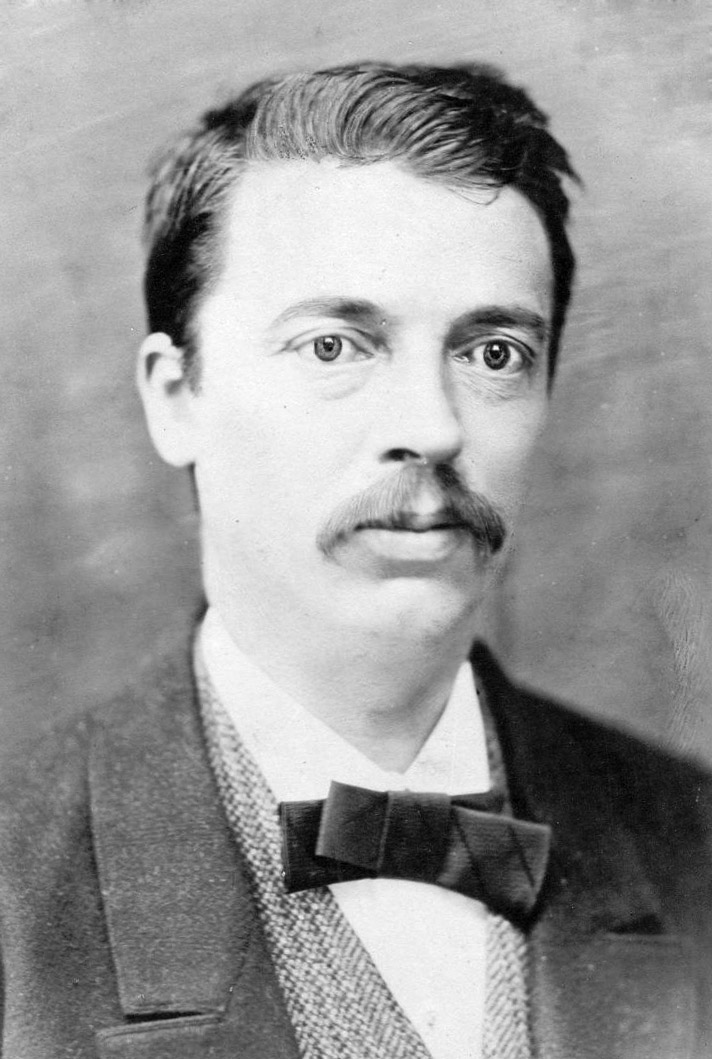
\includegraphics[width=4.182cm,height=6.186cm]{pictures/zulassungsarbeit-img012.jpg}

Abb. \stepcounter{Abb}{\theAbb}: August Högn &

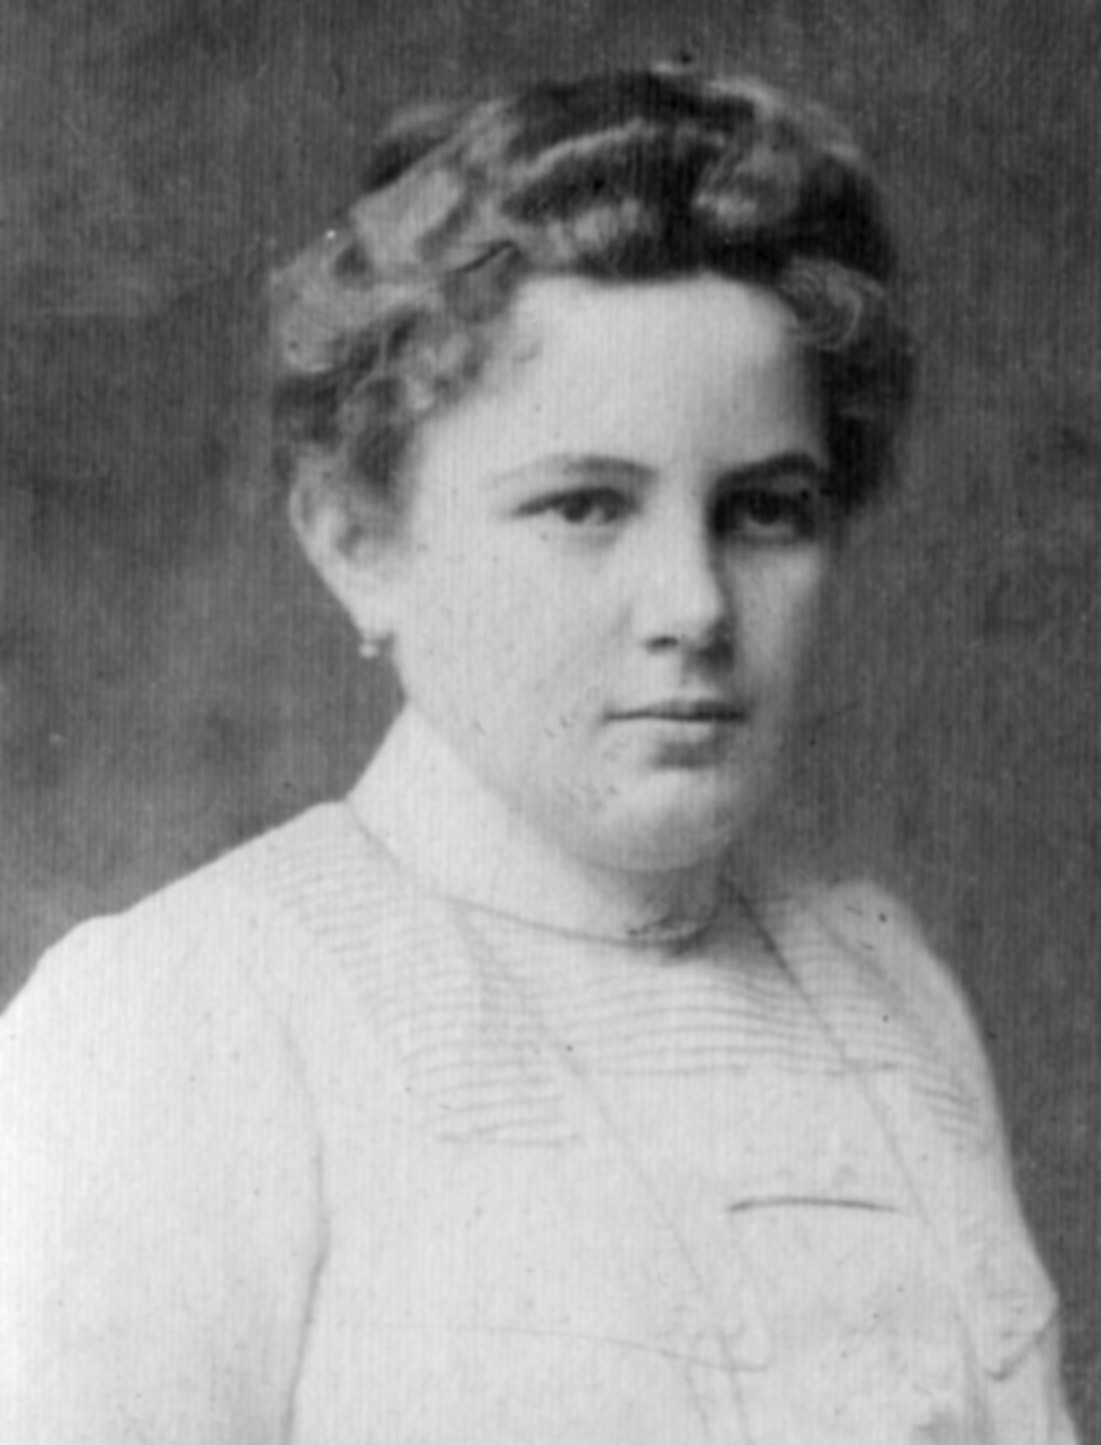
\includegraphics[width=4.711cm,height=6.189cm]{pictures/zulassungsarbeit-img013.jpg}

Abb. \stepcounter{Abb}{\theAbb}: Emma Högn &

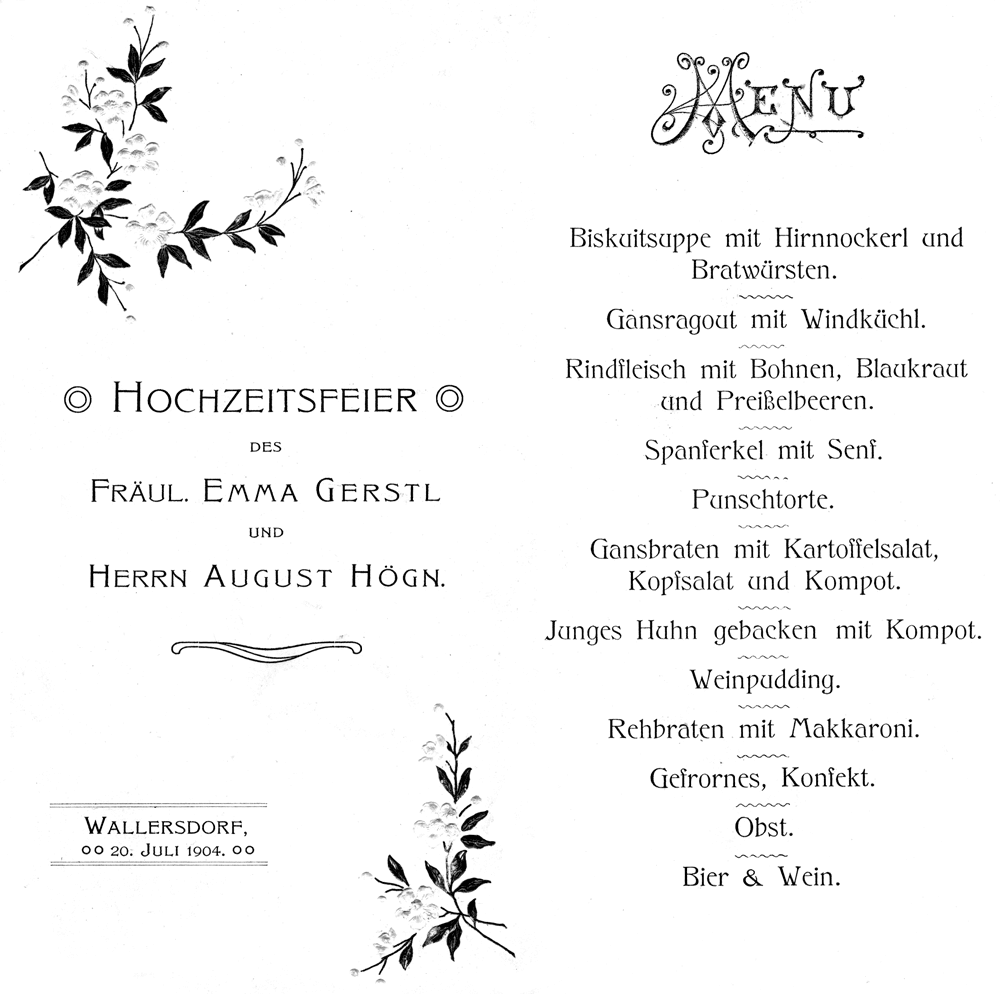
\includegraphics[width=6.218cm,height=6.179cm]{pictures/zulassungsarbeit-img014.png}

\label{bkm:Ref100297575}Abb. \stepcounter{Abb}{\theAbb}:
Hochzeitseinladung und Menü\\
\end{supertabular}
\end{flushleft}
Am 20. Juli 1904 fand in Wallersdorf die Hochzeit von August Högn und
der neun Jahre jüngern, damals 16-jährigen Emma Gerstl mit üppigem
Hochzeitsmenü statt, wie der Hochzeitseinladung (Abb. 12) entnommen
werden kann. \footnote{Dokument Nr. 111, Einladung zur Hochzeitsfeier,
20.7.1904} Emma Gerstl stammte aus einer wohlhabenden\footnote{
Interview Nr. 4, Maria Schröck, 30.12.2002, Absatz 4}
Bierbrauerfamilie,die in Gründobl, einem
kleinen Ort in der Nähe von Wallersdorf, ein großes Anwesen mit
Brauerei \footnote{Interview Nr. 21, Lilo Leuze, 2.12.2004, Absatz 20}
und Wirtshaus \footnote{Interview Nr. 3, Ida Högn, 29.12.2002, Absatz
36} besaß. Das junge Paar musste heiraten, da Emma Högn schwanger
wurde. Sie gebar Zwillinge, die beide kurz nach ihrer Geburt
starben. \footnote{Interview Nr. 3, Ida Högn, 29.12.2002, Absatz 36;
Interview Nr. 25, Lilo Leuze, 14.1.2005, Absatz 2} Zum 1. Juni 1905
wurde Högn nach Eberhardsreuth im Landkreis Grafenau
versetzt. \footnote{Dokument Nr. 48, Zeitungsartikel aus Viechtacher
Bayerwald-Bote, 2.8.1958} Hier kam die Tochter Elfriede, genannte
Frieda, am 14. August 1906 zur Welt. \footnote{Interview Nr. 20,
Gertraud von Molo, 23.11.2004, Absatz 6} Der Sohn Gustl erblickte am
17.1.1912 schon in Högns nächstem Einsatzort das Licht der Welt: in
Ruhmannsfelden. \footnote{Taufregister der Pfarrgemeinde St.
Laurentius, Ruhmannsfelden}

\begin{center}
\begin{minipage}{3.373cm}
\begin{center}
\tablefirsthead{}
\tablehead{}
\tabletail{}
\tablelasttail{}
\begin{supertabular}{m{3.1729999cm}}

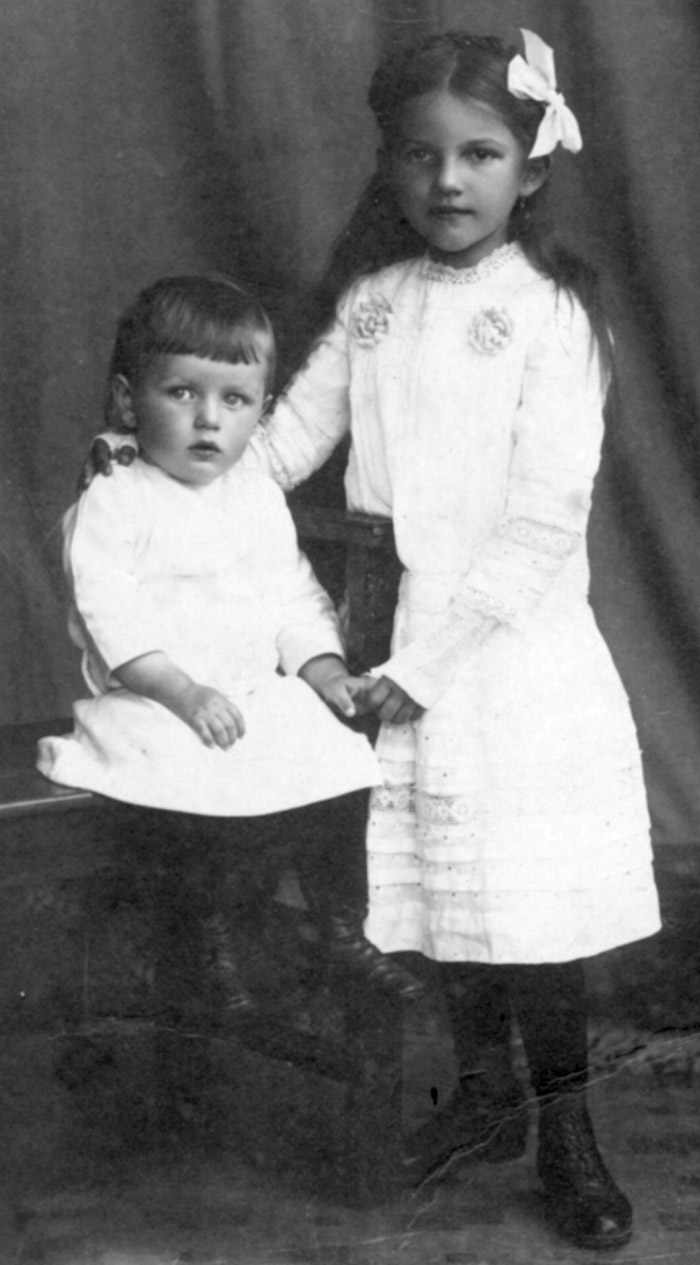
\includegraphics[width=2.99cm,height=5.408cm]{pictures/zulassungsarbeit-img015.jpg}

Abb. \stepcounter{Abb}{\theAbb}: Gustl und Frieda Högn\\
\end{supertabular}
\end{center}
\end{minipage}
\end{center}
